% VS Code Magic Command to use lualatex as the compiler
% !TeX program = lualatex

% Gemini theme
% https://github.com/anishathalye/gemini

\documentclass[final]{beamer}

% ====================
% Packages
% ====================

\usepackage[T1]{fontenc}
\usepackage{lmodern}
\usepackage[size=custom,width=100,height=75,scale=1.0]{beamerposter}
\usetheme{gemini}
\usecolortheme{umich}
\usepackage{graphicx}
\usepackage{booktabs}
\usepackage{tikz}
\usepackage{pgfplots}
\usepackage{subcaption}  % for figures with multiple images
\pgfplotsset{compat=1.14}

% ====================
% Lengths
% ====================

% If you have N columns, choose \sepwidth and \colwidth such that
% (N+1)*\sepwidth + N*\colwidth = \paperwidth
\newlength{\sepwidth}
\newlength{\colwidth}
\setlength{\sepwidth}{0.025\paperwidth}
\setlength{\colwidth}{0.3\paperwidth}

\newcommand{\separatorcolumn}{\begin{column}{\sepwidth}\end{column}}

% ====================
% Title
% ====================

\title{Some fancy title: followed by some more text 
      \newline a second line in the title}   % optionally, we can use two lines if the title is too long.

\author{Louise Belcher \inst{1} \and Fred Feng \inst{1}}

\institute[shortinst]{\inst{1} University of Michigan-Dearborn, Department of Industrial and Manufacturing Systems Engineering}
% \institute[shortinst]{\inst{1} Some Institute \samelineand \inst{2} Another Institute}

% ====================
% Footer (optional)
% ====================

\footercontent{
  Feng Group website: \href{https://fenggroup.org/}{https://fenggroup.org/} \hfill
  Transportation Research Board (TRB) Annual Meeting, 2025 \hfill
  Contact: Dr. Fred Feng at \href{mailto:fredfeng@umich.edu}{fredfeng@umich.edu}}
% (can be left out to remove footer)

% ====================
% Logo (optional)
% ====================

% use this to include logos on the left and/or right side of the header:
% \logoleft{
\includegraphics[height=10cm]{./images/umich.png}}
\logoleft{
\includegraphics[height=10cm]{./images/UMDearborn.png}}

\logoright{
\includegraphics[height=10cm]{./images/sure.png}}



% ====================
% Body
% ====================

\begin{document}

\begin{frame}[t]
\begin{columns}[t]
\separatorcolumn

\begin{column}{\colwidth}

  \begin{block}{A block title}

    Some block contents, followed by a figure, followed by a dummy paragraph.

    \begin{figure}
      \centering
        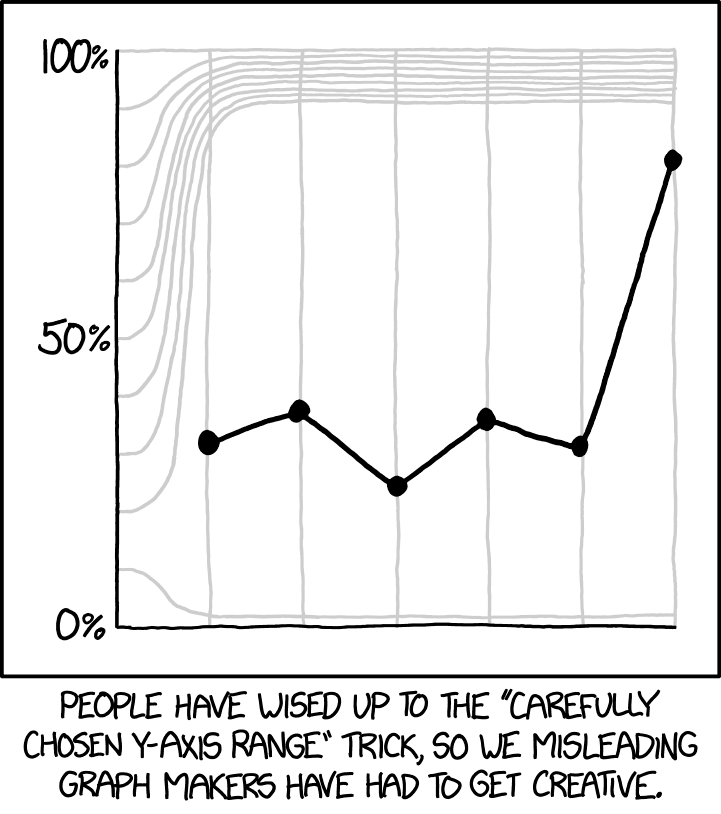
\includegraphics[width=.4\textwidth]{./images/y_axis_2x.png}
      \caption{XKCD Comic: Y-Axis (https://xkcd.com/2023/)}
    \end{figure}

    We can start each sentence with a new line.
    This style is helpful to spot and avoid writing very long sentences, which are harder to read.
    In the rendered document, a following sentence will follow the previous in the same paragraph.
    
    To start a new paragraph, simply add an empty line above the sentence.

  \end{block}

  \begin{block}{A block containing a list}

    An itemize (i.e., unordered) list is shown below. 

    \begin{itemize}
      \item \textbf{Mauris tempor} risus nulla, sed ornare
      \item \textbf{Libero tincidunt} a duis congue vitae
      \item \textbf{Dui ac pretium} morbi justo neque, ullamcorper
    \end{itemize}

    Some more text.

  \end{block}

  \begin{alertblock}{A highlighted block}

    This block catches your eye, so \textbf{important stuff} should probably go
    here.


    \begin{itemize}
      \item \textbf{Fusce dapibus tellus} vel tellus semper finibus. 
        In consequat, nibh sed mattis luctus, augue diam fermentum lectus.
      \item \textbf{In euismod erat metus} Vestibulum luctus augue in mi condimentum, at sollicitudin lorem viverra.
      \item \textbf{Suspendisse vulputate} mauris vel placerat consectetur.
        Mauris semper, purus ac hendrerit molestie, elit mi dignissim odio, in suscipit felis sapien vel ex.
    \end{itemize}

    Some more text.

  \end{alertblock}

\end{column}

\separatorcolumn

\begin{column}{\colwidth}

  \begin{block}{A block containing an enumerated list}

    An enumerated (i.e., ordered) list is shown below. 

    \begin{enumerate}
      \item The ingredients of a hamburger fall into place on a white screen, and Bob's hands appear underneath to hold it.
      \item The other family members appear around him one at a time, beginning with Linda and ending with Louise.
      \item Linda puts her arm around Bob, Tina stands expressionless, Gene plays a sound effect on his keyboard, and Louise poses for the camera.
    \end{enumerate}

  \end{block}

  \begin{block}{A block containing a figure with subfigures}

    A figure that contains a figure with subfigures.

    \begin{figure}
      \centering
      \begin{subfigure}{0.49\textwidth}
        \centering
        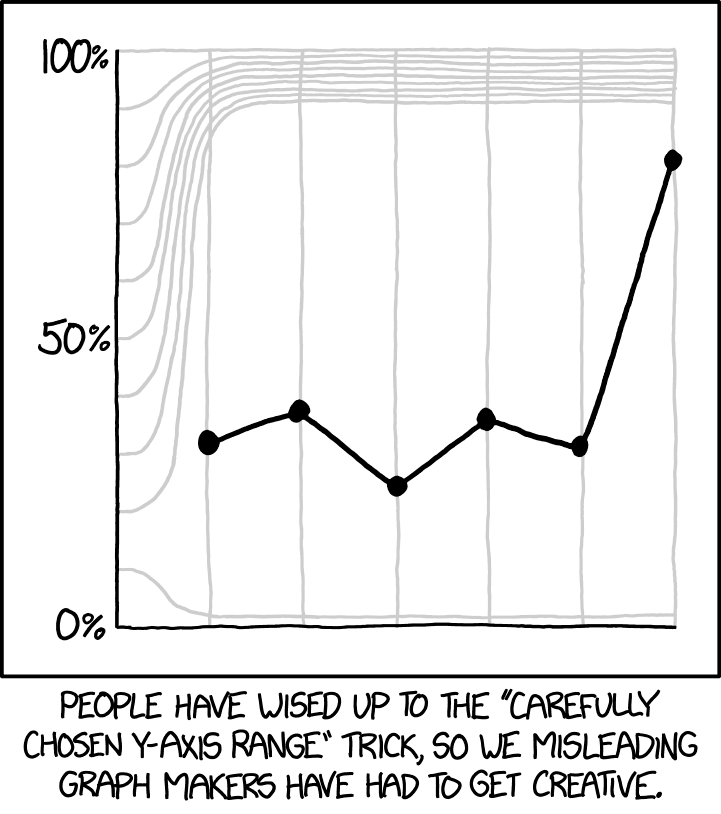
\includegraphics[height=15cm]{./images/y_axis_2x.png}
        \caption{caption for figure a}    % optional
      \end{subfigure}
      \hfill
      \begin{subfigure}{0.49\textwidth}
        \centering
        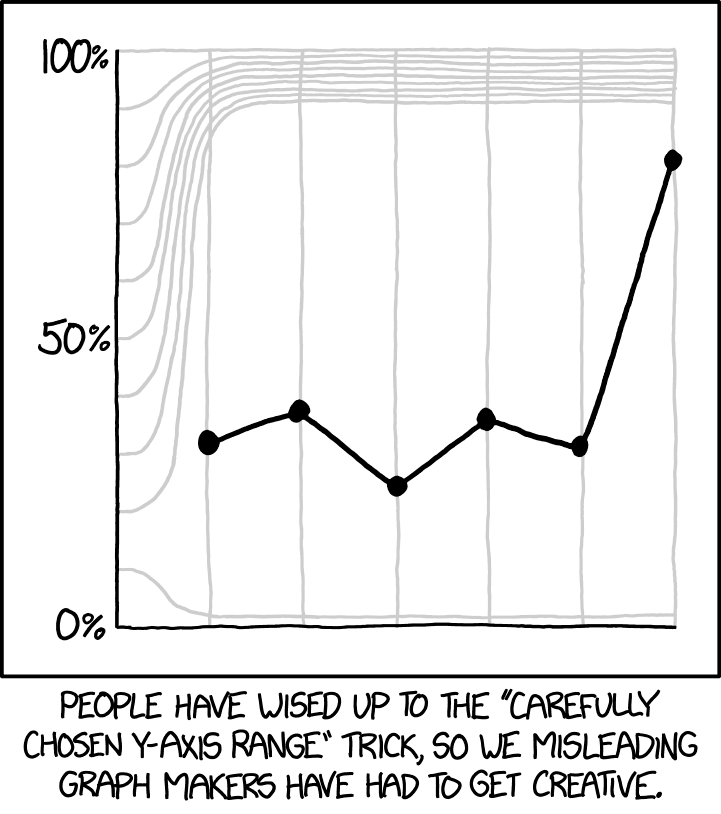
\includegraphics[height=15cm]{./images/y_axis_2x.png}
        \caption{caption for figure b}   % optional
      \end{subfigure}
      \caption{Caption for this figure}
    \end{figure}

  \end{block}

  \vspace{-1em}    % If needed, you can use vspace to manually adjust the vertical space.

  \begin{block}{A block containing nested lists}

    You can also format text \textit{with italic} or \textbf{bold fonts} to emphasize certain words.

    \begin{itemize}
      \item \textbf{Sed consequat} id ante vel efficitur. Praesent congue massa
        sed est scelerisque, elementum mollis augue iaculis.
        \begin{itemize}
          \item In sed est finibus, vulputate nunc gravida, pulvinar lorem.
          \item Fusce ornare dignissim nisi. 
          \item Donec rhoncus vestibulum erat, quis aliquam leo
            gravida egestas.
        \end{itemize}
      \item \textbf{Sed luctus, elit sit amet} dictum maximus, diam dolor
        faucibus purus, sed lobortis justo erat id turpis.
      \item \textbf{Pellentesque facilisis dolor in leo} bibendum congue.
        Maecenas congue finibus justo, vitae eleifend urna facilisis at.
    \end{itemize}

  \end{block}

\end{column}

\separatorcolumn

\begin{column}{\colwidth}

  \begin{exampleblock}{A highlighted block containing some math}

    A different kind of highlighted block.

    $$
    Y = \beta_0 + \beta_1 \cdot x + \epsilon
    $$

    Interdum et malesuada fames $\{x_1, x_2, \cdots, x_n \}$ ac ante ipsum primis in
    faucibus. Cras eleifend dolor eu nulla suscipit suscipit. Sed lobortis non
    felis id vulputate.

    \heading{A heading inside a block}

    Praesent consectetur mi $x^2 + y^2$ metus, nec vestibulum justo viverra
    nec. Proin eget nulla pretium, egestas magna aliquam, mollis neque. Vivamus
    dictum $\mathbf{u}^\intercal\mathbf{v}$ sagittis odio, vel porta erat
    congue sed. Maecenas ut dolor quis arcu auctor porttitor.

    \heading{Another heading inside a block}

    Sed augue erat, scelerisque a purus ultricies, placerat porttitor neque.
    Donec $P(y \mid x)$ fermentum consectetur $\nabla_x P(y \mid x)$ sapien
    sagittis egestas. Duis eget leo euismod nunc viverra imperdiet nec id
    justo.

  \end{exampleblock}

  \begin{block}{A block containing a table}

    See the table below:

    \begin{table}
      \centering
      \begin{tabular}{l r r c}
        \toprule
        \textbf{First column} & \textbf{Second column} & \textbf{Third column} & \textbf{Fourth} \\
        \midrule
        Foo & 13.37 & 384,394 & $\alpha$ \\
        Bar & 2.17 & 1,392 & $\beta$ \\
        Baz & 3.14 & 83,742 & $\delta$ \\
        Qux & 7.59 & 974 & $\gamma$ \\
        \bottomrule
      \end{tabular}
      \caption{A table caption.}
    \end{table}

    Donec quis posuere ligula. Nunc feugiat elit a mi malesuada consequat. Sed
    imperdiet augue ac nibh aliquet tristique. Aenean eu tortor vulputate,
    eleifend lorem in, dictum urna. Proin auctor ante in augue tincidunt
    tempor. Proin pellentesque vulputate odio, ac gravida nulla posuere
    efficitur. Aenean at velit vel dolor blandit molestie. Mauris laoreet
    commodo quam, non luctus nibh ullamcorper in. Class aptent taciti sociosqu
    ad litora torquent per conubia nostra, per inceptos himenaeos.

    Nulla varius finibus volutpat. Mauris molestie lorem tincidunt, iaculis
    libero at, gravida ante. Phasellus at felis eu neque suscipit suscipit.
    Integer ullamcorper, dui nec pretium ornare, urna dolor consequat libero,
    in feugiat elit lorem euismod lacus. Pellentesque sit amet dolor mollis,
    auctor urna non, tempus sem.

  \end{block}

  \begin{block}{References}

    \nocite{*}   % adds everything in the bib file to the bibliography
    \footnotesize{\bibliographystyle{plain}\bibliography{poster}}

  \end{block}

\end{column}

\separatorcolumn
\end{columns}
\end{frame}

\end{document}
